\defcitealias{Tarango-Yong:2018a}{Paper~I}
\newcommand\PaperI{\citetalias{Tarango-Yong:2018a}}

\section{Introduction}
\label{sec:introduction}
\newcommand\hii{\ion{H}{ii}}

Curved emission arcs around stars \citep[e.g.,][]{Gull:1979a} are
often interpreted as \textit{bow shocks}, due to a supersonic
hydrodynamic interaction between the star's wind and an external
stream. This stream may be due to the star's own motion or to an
independent flow, such as an \hii{} region in the champagne phase
\citep{Tenorio-Tagle:1979a}, or another star's wind
\citep{Canto:1996}. However, an alternative interpretation in some
cases may be a radiation-pressure driven bow wave, as first proposed
by \citet[\S\textsc{vi}]{van-Buren:1988a}.  In this scenario, photons
emitted by the star are absorbed by dust grains in the incoming
stream, with the resultant momentum transfer being sufficient to
decelerate and deflect the grains within a certain distance from the
star, forming a dust-free, bow-shaped cavity with an enhanced dust
density at its edge.  Two regimes are possible, depending on the
strength of coupling between the gas (or plasma) and the dust.  In the
strong-coupling regime, gas--grain drag decelerates the gas along with
the dust, forming a shocked gas shell in a similar fashion to the
wind-driven bow shock case.  In the weak-coupling regime, the gas
stream is relatively unaffected and the dust temporarily decouples to
form a dust-only shell.  This second case has recently been studied in
detail in the context of the interaction of late O-type stars (which
have only weak stellar winds) with dusty photoevaporation flows inside
\hii{} regions \citep{Ochsendorf:2014a, Ochsendorf:2014b,
  Ochsendorf:2015a}.  We follow the nomenclature proposed by
\citet{Ochsendorf:2014b}, in which \textit{dust wave} refers to the
weak coupling case and \textit{bow wave} to the strong coupling case.
More complex, hybrid scenarios are also possible, such as that studied
by \citet{van-Marle:2011a}, where a hydrodynamic bow shock forms, but
the larger dust grains that accompany the stellar wind pass right
through the shocked gas shell, and form their own dust wave at a
larger radius.

\begin{figure}
  \centering
  \framebox{
    \parbox[m][4cm]{0.8\linewidth}
    {\centerline{\textbf{\dotfill TODO\dotfill}}}}
  \caption{Bow shocks, bow waves, and dust waves}
  \label{fig:3-types-bow}
\end{figure}

In \citet[][hereafter \PaperI{}]{Tarango-Yong:2018a}, we proposed a
new two-dimensional classification scheme for bow shapes: the
projected planitude--alatude, or \(\Pi'\)--\(\Lambda'\), diagram.  Planitude
measures the flatness of the bow's apex, while alatude measures the
openness of the bow's wings.  Both are dimensionless ratios of lengths
that can be estimated from observational images.  We have analyzed the
inclination-dependent tracks on the \(\Pi'\)--\(\Lambda'\) plane for simple
geometric shapes (spheroids, paraboloids, hyperboloids) and for
thin-shell hydrodynamic bow shock models (wilkinoid, cantoids,
ancantoids).  In this paper, we will do the same for simple models of
radiation-driven dust waves (dragoids) and bow waves (trapoids).

The paper is organized as follows.
%
In \S~\ref{sec:shape-dust-wave} we do the same for simple models of a
dusty radiation bow wave (dragoids), including the effects of
gas-grain drag.
%
In \S~\ref{sec:perturbed-bows} we investigate the effects on the
planitude--alatude plane of small-amplitude perturbations to the bow
shape.
%


\section{Different types of bow}
\label{sec:different-types-bow}

\begin{figure*}
  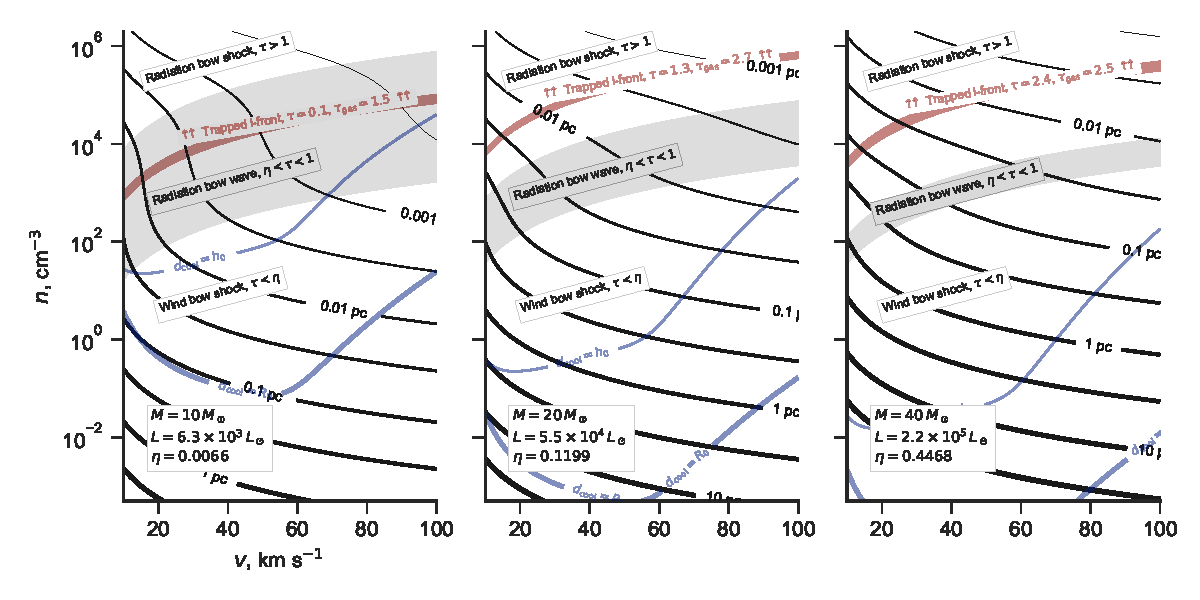
\includegraphics[width=\linewidth]{figs/zones-v-n-plane}
  \caption{Bow regimes in parameter space (\(v, n\)) of the external
    stream for main-sequence OB stars of different masses:
    (a)~\SI{10}{M_\odot}, (b)~\SI{20}{M_\odot}, (c)~\SI{40}{M_\odot}.  In all
    cases, \(\kappa = \SI{600}{cm^2.g^{-1}}\) and efficient gas-grain
    coupling is assumed. Solid black lines of varying width show the
    bow size (star-apex separation, \(R_0\)), while gray shading shows
    the radiation bow wave regime, with lower border \(\tau = \eta\) and
    upper border \(\tau = 1\), where \(\tau = 2 \kappa \rho R_0\) is the optical
    depth through the bow.  For bows above the red solid line, the
    ionization front is trapped inside the bow.  Blue lines delineate
    different cooling regimes.  Above the thin blue line
    (\(d_{\text{cool}} = h_0\)), the bow shock radiates efficiently,
    forming a thin shocked shell.  Below the thick blue line
    (\(d_{\text{cool}} = R_0\)), the bow shock is essentially
    non-radiative.}
  \label{fig:zones-v-n-plane}
\end{figure*}

In this section, we investigate the different types of bow interaction
that will occur in different regions of parameter space. We will
mainly treat the canonical case\footnote{%
  Variant cases with differing arrangements of dust and radiation
  sources are treated in \S~\ref{sec:case-inside-out}.} %
of a bow around a star of bolometric luminosity, \(L\), with a
radiatively driven wind, which is immersed in an external stream of
gas and dust with density, \(\rho\), and velocity, \(v\).  The size and
shape of the bow is determined by a generalized balance of pressure
(or, equivalently, momentum) between internal and external sources.
We assume that the stream is supersonic and super-alfvenic, so that
the external pressure is dominated by the ram pressure: \(\rho v^2\).

\subsection{Strong gas-grain coupling}
\label{sec:strong-gas-grain}

We first consider the case where the dust grains and gas are perfectly
coupled by collisions.\footnote{%
  Cases where this assumption does not hold are investigated below in
  \S~\ref{sec:imperf-coupl-betw}.} %
Although dust grains typically constitute only a small fraction
\(Z\grain \sim 0.01\) of the mass of the external stream, they
nevertheless dominate the broad-band opacity at FUV, optical and IR
wavelengths if they are present.\footnote{%
  At EUV wavelengths (\(\lambda < \SI{912}{\angstrom}\)), gas opacity
  dominates if the hydrogen neutral fraction is larger than
  \(\approx 0.001\), see discussion of ionization front trapping
  below.} %
The strong coupling assumption means that all the radiative forces
applied to the dust grains are directly felt by the gas also.

The internal pressure is the sum of wind ram pressure and the
effective radiation pressure that acts on the bow shell.  The
radiative momentum loss rate of the star is \(L/c\) and the wind
momentum loss rate can be expressed as
\begin{equation}
  \label{eq:wind-efficiency}
  \dot{M} V = \eta L / c \ , 
\end{equation}
where \(\eta\) is the momentum efficiency of the wind, which is typically
\(< 1\) \citep{Lamers:1999b}. If the optical depth is very large, then
all of the stellar radiative momentum, emitted with rate \(L/c\), is
trapped by the bow shell.  In the single scattering limit,\footnote{%
  Although it may seem inconsistent to assume single scattering in the
  case of high optical depths, this is defensible for the following
  reasons. (1)~The grain albedo is not that high (typically
  \(\sim 0.5\) at ultraviolet through optical wavelengths). (2)~The
  scattered radiation field is more isotropic than the stellar field,
  leading to cancellation in the radiative
  flux. (3)~Absorbed radiation is re-emitted at infrared
  wavelengths, where the dust opacity is very much lower.} %
and temporarily neglecting the wind, then pressure balance at the bow
apex, a distance \(R_0\) along the symmetry axis from the star is
given by
\begin{equation}
  \label{eq:rad-press-balance-thick}
  \frac{L}{4 \pi c R_0^2} = \rho v^2 \ ,
\end{equation}
which yields a fiducial bow shock radius in this optically thick limit
as
\begin{equation}
  \label{eq:Rstar}
  R_* = \left(\frac{L}{4\pi c \rho v^2}\right)^{1/2} \ .
\end{equation}

We now consider the opposite, optically thin limit.  If the total
opacity (gas plus dust) per total mass (gas plus dust) is \(\kappa\) (with
units of \si{cm^2.g^{-1}}), then the radiative acceleration is
\begin{equation}
  \label{eq:rad-accel}
  a_{\text{rad}} = \frac{\kappa L}{4 \pi c R^2} \ , 
\end{equation}
so that an incoming stream with initial velocity, \(v_\infty\), can be
brought to rest by radiation alone\footnote{%
  For simplicity, we here ignore the effects of pressure gradients and
  shocks, which are important as the velocity approaches the sound
  speed, \(\sound\). In \S~XX below, we show that the resultant
  corrections to \(R_0\) are of order \(\sound / v_\infty\).} %
at a distance \(R_0\) where
\begin{equation}
  \label{eq:rad-poten}
  \int_{R_0}^\infty a_{\text{rad}} \, dr = \tfrac12 v^2 \ , 
\end{equation}
yielding
\begin{equation}
  \label{eq:rad:R0}
  R_0 = \frac{\kappa L}{2\pi c v_\infty^2} \ .
\end{equation}
On the other hand, we can also argue as in the optically thick case
above by approximating the bow shell as a surface, and balancing
stellar radiation pressure against the ram pressure of the incoming
stream.  The important difference when the shell is not optically
thick is that only a fraction \(1 - e^{-\tau}\) of the radiative momentum
is absorbed by the bow, so that
equation~\eqref{eq:rad-press-balance-thick} is replaced with
\begin{equation}
  \label{eq:rad-press-balance-tau}
  \frac{L (1 - e^{-\tau})}{4 \pi c R_0^2} = \rho v^2 \ .
\end{equation}
In the optically thin limit, \(1 - e^{-\tau} \approx \tau\), so these two
descriptions can be seen to agree so long as
\(\tau = 2 \kappa \rho R_0\), which we will assume to hold generally.

Then, defining a fiducial optical depth, \(\tau_* = \rho \kappa R_*\), and adding
in the stellar wind ram pressure\footnote{%
  We implicitly assume that the interaction of the stellar wind with
  the external stream can always be treated in the continuum limit.
  This will be true if either the collisional mean free path or the
  ion Larmor radius is much smaller than \(R_0\), which is almost
  always the case.} %
from equation~\eqref{eq:wind-efficiency}, we find that the general bow
radius can be written in terms of the fiducial radius as
\(R_0 = x R_*\), where \(x\) is the solution of
\begin{equation}
  \label{eq:rad-full-x}
  x^2 - \bigl(1 - e^{-2 \tau_* x} \bigr) - \eta = 0 \ .
\end{equation}
Since this is a transcendental equation, \(x\) must be found
numerically, but we can write explicit expressions for three limiting
cases:
\begin{equation}
  \label{eq:x-cases}
  x \approx
  \begin{cases}
    \text{if \(\tau_* \gg 1\):} & (1 + \eta)^{1/2}  \\
    \text{if \(\tau_*^2 \ll 1\):} & \tau_* + \bigl( \tau_*^2 + \eta \bigr)^{1/2} \approx
    \begin{cases}
      \text{if \(\tau_*^2 \gg \eta\):} & 2 \tau_*  \\
      \text{if \(\tau_*^2 \ll \eta\):} & \eta^{1/2} 
    \end{cases}
  \end{cases}
\end{equation}
The first case, \(x \approx (1 + \eta)^{1/2}\), corresponds to a
\textit{radiation bow shock}; the second case,
\(x \approx 2 \tau_* \), corresponds to a \textit{radiation bow wave}; and the
third case, \(x \approx \eta^{1/2}\), corresponds to a \textit{wind bow shock}.
The two bow shock cases are similar in that the external stream is
oblivious to the presence of the star until it suddenly hits the bow
shock shell, differing only in whether it is radiation or wind that is
providing the internal pressure.  In the intermediate bow wave case,
on the other hand, the external stream is gradually decelerated by
absorption of photons as it approaches the bow.\footnote{A shock does
  still form in this case, but shocked material constitutes a small
  fraction of the total column density of the shell, see
  \S~\ref{sec:shape-bow-wave}.}

\begin{table*}
  \centering
  \caption{Stellar parameters for example stars}
  \label{tab:stars}
  \begin{tabular}{l S S S S S S S S S l}
    \toprule
    & {\(M / \si{M_\odot}\)} & {\(L_4\)}
    & {\(\dot{M}_{-7}\)} & {\(V_3\)} & {\( \eta \)}
    & {Sp.~Type} 
    & {\(T_{\text{eff}} / \si{kK}\)} & {\(\lambda_{\text{eff}}\) / \si{\um}}
    & {\(S_{49}\)} & Figures 
    \\
    \midrule
    & 10 & 0.63 & 0.0034 & 2.47 & 0.0066 & {B1.5\,V} & 25.2 & 0.115 & e-4
                   & \ref{fig:zones-v-n-plane}a,
                     \ref{fig:decouple-v-n-plane},
                     \ref{fig:decouple-v40-versus-n} \\
    Main-sequence OB stars
    & 20 & 5.45 & 0.492 & 2.66 & 0.1199 & {O9\,V} & 33.9 & 0.086 & 0.1
                   & \ref{fig:zones-v-n-plane}b\\
    & 40 & 22.2 & 5.1 & 3.31 & 0.4468 & {O5\,V} & 42.5 & 0.068 & 1.0
                   & \ref{fig:zones-v-n-plane}c\\[\smallskipamount]
    Red supergiant star
    & 20 & 15.6 & 100 & 0.015 & 0.0476 & {M1\,Ia} & 3.6 & 0.805 & 0
                   & \\ 
    \bottomrule
  \end{tabular}
\end{table*}

We now consider the application to bow shocks around main sequence OB
stars, expressing stellar and ambient parameters in terms of typical
values as follows:
\begin{gather*}
  \label{eq:stellar-parameters}
  \dot{M}_{-7} = \dot{M} / \bigl(\SI{e-7}{M_\odot.yr^{-1}}\bigr) \\
  V_3 = V / \bigl(\SI{1000}{km.s^{-1}}\bigr) \\
  L_4 = L / \bigl(\SI{e4}{L_\odot}\bigr) \\
  v_{10} = v_\infty / \bigl( \SI{10}{km.s^{-1}} \bigr) \\
  n = (\rho / \bar{m}) / \bigl( \SI{1}{cm^{-3}} \bigr) \\
  \kappa_{600} = \kappa / \bigl( \SI{600}{cm^2.g^{-1}} \bigr) \ ,
\end{gather*}
where \(\bar{m}\) is the mean mass per hydrogen nucleon
(\(\bar{m} \approx 1.3 m_{\text{p}} \approx \SI{2.17e-24}{g}\) for solar
abundances).  Note that \(\kappa = \SI{600}{cm^2.g^{-1}}\) corresponds to a
cross section of \(\approx \SI{e-21}{cm^2}\) per hydrogen nucleon, which is
typical for interstellar medium dust \citep{Bertoldi:1996a} at far
ultraviolet wavelengths, where OB stars emit most of their radiation.
In terms of these parameters, we can express the stellar wind momentum
efficiency as
\begin{equation}
  \label{eq:wind-eta-typical}
  \eta = \num{0.495} \,\dot{M}_{-7} \,V_3  \,L_4^{-1}
\end{equation}
and the fiducial radius and optical depth as
\begin{align}
  \label{eq:fiducial-typical}
  R_* / \si{pc} &= \num{2.21} \, (L_4 / n)^{1/2} \,v_{10}^{-1} \\
  \tau_* &= \num{0.0089} \,\kappa_{600} \, (L_4 \,n)^{1/2} \,v_{10}^{-1} \ .
\end{align}
In Figure~\ref{fig:zones-v-n-plane}, we show results for the bow size
(apex distance, \(R_0\)) as a function of the density, \(n\), and
relative velocity, \(v_\infty\), of the external stream, with each panel
corresponding to a particular star, with parameters as shown in
Table~\ref{tab:stars}.  To facilitate comparison with previous work,
we choose stellar parameters similar to those used in the
hydrodynamical simulations of \citet{Meyer:2014b, Meyer:2016a,
  Meyer:2017a}, based on stellar evolution tracks for stars of
\SIlist{10;20;40}{M_\odot} \citep{Brott:2011a} and theoretical wind
prescriptions \citep{de-Jager:1988a, Vink:2000a}.  Although the
stellar parameters do evolve with time, they change relatively little
during the main-sequence lifetime of several million years.\footnote{%
  \label{fn:meyer-velocities-too-low}
  Note that we have recalculated the stellar wind terminal velocities,
  since the values given in the \citeauthor{Meyer:2014b} papers are
  troublingly low.  We have used the prescription
  \(V = 2.6 V_{\text{esc}}\), where
  \(V_{\text{esc}} = \left( 2 G M (1 - \Gamma_e)/ R \right)^{1/2}\) is the
  photospheric escape velocity, which is appropriate for strong
  line-driven winds with \(T_{\text{eff}} > \SI{21 000}{K}\)
  \citep{Lamers:1995a}.  We find velocities of
  \SIrange{2500}{3300}{km.s^{-1}}, which are consistent with
  observations and theory \citep{Vink:1999a} for O~stars, but at least
  two times higher than those cited by \citet{Meyer:2014b}. For
  main-sequence B~stars, wind column densities are too low to reliably
  measure the terminal velocity from near ultraviolet P~Cygni profiles
  \citep{Prinja:1989a}, and so the values are theory-dependent
  \citep{Krticka:2014a} and hence more uncertain.  A further
  complication is the existence of a subset of OB stars with
  anomalously weak winds \citep{Puls:2008a}, which in some cases is
  related to the presence of strong (\(\sim \SI{1}{kG}\)) magnetic fields
  \citep{Oskinova:2011b}.} %
The three examples are an early B~star (\SI{10}{M_\odot}), a late O~star
(\SI{20}{M_\odot}), and an early O~star (\SI{40}{M_\odot}), which cover the
range of luminosities and wind strengths expected from bow-producing
hot main sequence stars.  The luminosity is a steep function of
stellar mass (\(L \sim M^{2.5}\)) and the wind mass-loss rate is a steep
function of luminosity (\(\dot{M} \sim L^{2.2}\)), which means that the
wind momentum efficiency is also a steep function of mass
(\(\eta \sim M^3\)), approaching unity for early O~stars, but falling to
less than 1\% for B~stars.


\subsection{Imperfect coupling between gas and dust}
\label{sec:imperf-coupl-betw}

\begin{figure}
  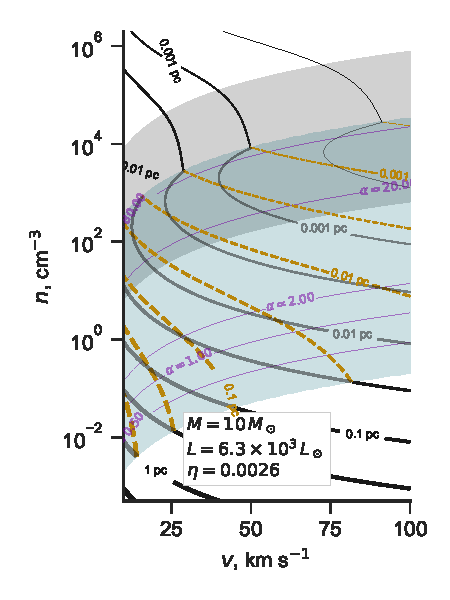
\includegraphics[width=\linewidth]{figs/decouple-v-n-plane}
  \caption{As Fig.~\ref{fig:zones-v-n-plane}(a), but accounting for
    gas-grain decoupling with constant efficiency \(\xi = 0.07\). }
  \label{fig:decouple-v-n-plane}
\end{figure}

\begin{figure}
  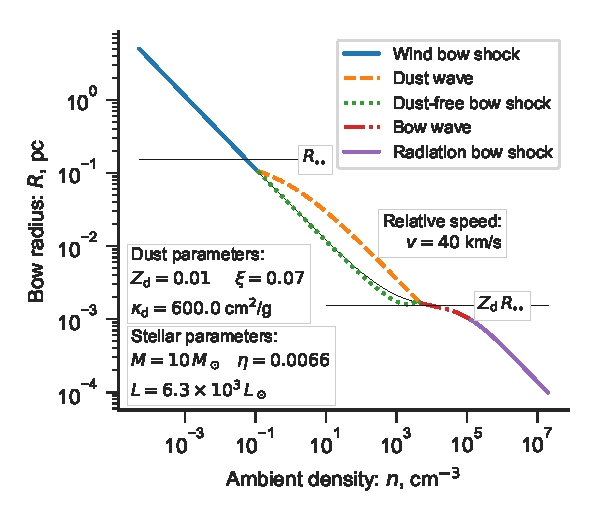
\includegraphics[width=\linewidth]{figs/decouple-v40-versus-n}
  \caption{Vertical cut through Fig.~\ref{fig:decouple-v-n-plane},
    showing bow radius and different regimes for a fixed inflow
    velocity of \SI{40}{km.s^{-1}}.}
  \label{fig:decouple-v40-versus-n}
\end{figure}


\subsection{The case of inside-out bows}
\label{sec:case-inside-out}

So far, we have considered the case where the inner source dominates
the radiation, while dust is present only in the outer stream, which
applies to hot stars interacting with the ISM.  However, in the case
of cool stars, the inner wind will also be dusty.  Examples are the
red supergiant (RSG) phase of high-mass evolution, or the asymptotic
giant branch (AGB) stage of low/intermediate-mass evolution.  In both
these cases, it is still the inner source that provides the radiation
field.  However, not all winds are radiatively driven and in those
cases it is conceivable that it is the outer source that dominates the
radiation field.  An example is the case of photoevaporating
protoplanetary disks (proplyds) in the Orion Nebula and other \hii{}
regions \citep{ODell:1994a}.  In the proplyds, the inner wind is a
thermally driven photoevaporation flow \citep{HA:1998, Henney:1999a},
while the outer stream is the stellar wind from an O~star
\citep{Garcia-Arredondo:2001a}.


%%% Local Variables:
%%% mode: latex
%%% TeX-master: "dusty-bow-wave"
%%% End:
